\documentclass[../main.tex]{subfiles}

\begin{document}

\chapter{Như Huy khai vỡ hiện thực như thực từ giữa những câu phức}

\begin{metadata}

\begin{flushright}5.4.2008\end{flushright}

Inrasara 



\end{metadata}

\begin{multicols}{2}

\begin{figure}
	\centering
	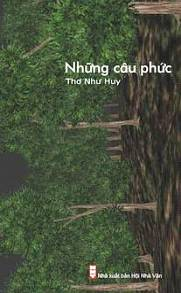
\includegraphics[width=\textwidth]{../img/tho050408.jpg}
	\caption{
\textit{Những câu phức}, thơ Như Huy, Nhà xuất bản Hội Nhà văn, 2008}
\end{figure}
     \begin{blockquote}
 
\textit{“Giữa những khe hẹp và sâu của vô số lớp hiện thực…”} 

\end{blockquote}
 
Hắn rơi và chìm dưới vực thẳm của nỗi vong thân. Hắn biết hắn không là cái này, không là cái kia hay cái nào khác bất kì. Mà “là-một-cá-nhân”. Hắn cựa quậy. Hắn bơi chới với giữa vô số bóng ma tha nhân, bóng ma “chúng ta”. 
\begin{blockquote}
 
\textit{“Trong một thời đại mà lời bị che khuất bởi hình ảnh được kiến tạo của lời, hiện thực bị che khuất bởi ý muốn của chúng ta về hiện thực…} 

\end{blockquote}
 
Tại sao? Tại sao? Tại sao? Hắn thức nhận thẳm sâu rằng cuộc sống lâu nay hắn sống chỉ là nỗi giả tạo và giả vờ. Hắn bắt đầu nổi loạn và quyết làm cuộc chinh phục tự do. Nhưng:  
\begin{blockquote}
 
\textit{“Cái anh chọn lựa rốt cục không phải là những gì anh muốn, mà là những gì cả anh và họ cùng giả vờ tin.”} 

\end{blockquote}
 
Khởi đầu biết suy nghĩ là khởi đầu vong thân. Nổi loạn hay không nổi loạn, chúng ta vẫn mắc kẹt vào đống hỗn độn của một hiện thực giả tạo. Hiện thực giả tạo được tạo nên bởi vô số giải trình ngôn ngữ – ngôn ngữ giả tạo. Của muôn ngàn thế hệ trước, của thế hệ ta đang sống, của người khác và chính ta. 
 
Rơi và chìm giữa hiện thực giả tạo đó, Như Huy đã làm gì? 
 
Anh làm mấy cuộc khai phá! Với một công cụ duy nhất: sự tự thức, tự tri, một ý thức phản tỉnh (self conciousness), anh đào bới và khuấy tung tất cả. Để nhìn/tìm lại... 
 
 
\textbf{bản chất ngôn ngữ}… 
 
Ở khe hẹp “hai câu phức”, trong một “từ” vô nghĩa, nơi một “chữ thuần túy” hay giữa “các chữ”. Bất lực, vô nghĩa và ngu xuẩn. Ngôn ngữ bất lực và ta biết ta ngu xuẩn. Ta rối mù giữa cõi hỗn mang chữ. Giải trình tiếp nối giải trình, giải trình chống lại hay hùa theo giải trình, giải trình này ảo tưởng vượt mặt giải trình kia bằng một giải trình khác nữa nhưng nó vẫn là một giải trình. Không hơn kém phân tấc. Cứ thế! Chúng cuốn con người vào vòng xoáy vô cùng tận của chúng. 
 
Bởi, khởi sự suy tư là bắt đầu vướng vào ngôn ngữ. Con người suy tư qua, với và bằng ngôn ngữ. Làm sao vượt thoát khỏi chúng? Nói như Như Huy: làm sao để “ngôn ngữ là…”? Hay như Heidegger, làm thế nào suy tưởng mà không vướng lụy tư tưởng [bằng] biểu tượng (representational thought), để kẻ suy tư có thể bước lên con đường – nơi đó, ngôn ngữ sẽ là ngôn ngữ của Tính thể, như những đám mây là những đám mây của bầu trời? (“In this way language is the language of Being, as clouds are the clouds of the sky” -  M. Heidegger, \textit{Letter on Humanism}, bản dịch của Frank A. Capuzzi, trong \textit{Basic Writings}, Harper San Francisco, USA, 1977, p. 242). 
 
Khám phá tương quan giữa ngôn ngữ và con người, sự vận hành của ngôn ngữ trong tâm thức con người, tác động của nó lên suy tư và hoạt động của con người, là khởi đầu quan trọng.  
 
Như Huy tiếp tục truy tìm\textit{… }\textbf{bản chất bài thơ,}\textit{ c}ùng phương thức như đã.  
 
Từ bài thơ đầu [tiên, đời]: “Một-bài-thơ-đi-qua-khung-cửa…” bất chợt, đầy bản năng, ngây thơ và phiêu lãng. Nhưng khi kẻ làm thơ ý thức về việc làm thơ và bài thơ là hắn đánh mất bản thể mình ngay lúc đó.\textit{ Kẻ-Chia-Ngôn-Ngữ-Và-Hiện-Thực-Làm-Hai; Kẻ, Vì-Đánh-Mất-Hiện-Thực-Nên-Đánh-Mất-Luôn-Ngôn-Ngữ; Kẻ-Đã-Lẩn-Hẳn-Vào-Mặt-Nạ-Của-Chính-Mình.} 
 
Nhà thơ bị ném vào cõi rối mù của vô vàn giải trình, chịu ma sát giữa những chọn lựa, cái này cái kia hay cái khác nữa. Hắn nhận thấy hắn chỉ là một ảo ảnh, ảo ảnh thuần túy. Làm sao có thể tác thi mà không bị vướng kẹt vào giải trình? Bất khả. Làm sao khôi phục lại “Một bài thơ”? Một bài thơ \textit{như là} một bài thơ luôn chính là… 
 
Đây là một câu hỏi lớn. 
 
Như Huy dấn mình vào khảo sát sự thể gần gũi và cụ thể hơn: \textbf{bản chất tình yêu.} Nhưng khi đối mặt với sự thể đầy nhiêu khê này, sự tra vấn hứa hẹn sẽ khó khăn và quyết liệt hơn. Làm sao thi sĩ có thể giáp mặt nó mà không phải giẫm lên con đường mòn thiên hạ đã từng đi, đến nhàm sáo? Anh cần tiếp cận đa chiều, vận dụng nhiều biện pháp. Từ lật lại cuộc tình lớn và bi đát nơi sương mù lịch sử đất nước: Nguyễn Trãi và Nguyễn Thị Lộ đến khai mở đối thoại siêu hình trong truyền thống văn chương phương Tây: Faust và Gretchen, từ \textit{“mô tả tình yêu từ những khuôn mặt”} đến \textit{“mô tả tình yêu từ những cảm giác sinh lí”}, hay cả từ một bài thơ về tình yêu,… tất tần tật. Như Huy ngộ ra rằng dẫu cặp tình nhân\textit{ “đời đời trong nỗi khát khao vươn ra chạm vào một khuôn mặt khác”} nhưng, họ vẫn cứ giả tạo và bất lực. \textit{Tất-Thẩy-Đều-Xa-Lạ}.         
\begin{blockquote}
 
\textit{“cơ thể này chưa là chúng ta, cơn đau này chưa là chúng ta”} 

\end{blockquote}
 
Tôi yêu em là yêu hình ảnh phóng chiếu từ ý tưởng tôi về em, hơn thế nữa – từ ngôn ngữ tôi về em, từ bài thơ tình của tôi về em. Nghĩa là tôi yêu tôi. Tình yêu chỉ còn là một sở hữu, đơn và thuần. Sở hữu cái Tôi, sở hữu chính ngôn ngữ tôi về em. Khốn khổ thay! Vậy làm sao có thể tìm thấy nhau, trong tình yêu thuần khiết, tinh khôi không qua sương mù hồi ức? Khác đi, làm sao có thể vượt qua những câu phức, muôn ngàn câu phức hỗn độn trong suốt tập thơ hỗn mang này? Để có thể  tái thiết lại tình yêu, từ đó \textit{“tái thiết lại thế giới và hiện thực”}. Không có cách gì hơn là làm cuộc nhảy, bằng dũng cảm đánh cắp,\textit{ “cướp đi trọn vẹn nguồn từ vựng”} của nhau. Của anh và của em. Chỉ thế thôi, ta mới hi vọng \textit{Trông-Rõ-Khuôn-Mặt-Nhau}. Để tình yêu hiện thể như là thế. Và hiện thực hiện ra với chúng ta như là hiện thực. 
 
Như Huy đề nghị “một bộ ngữ pháp lạ lùng”. Một mơ mộng khác – như Rimbaud đã từng mơ mộng [Truy tìm một ngôn ngữ… thứ ngôn ngữ trực tiếp từ tâm hồn đi đến tâm hồn: Trouver une langue… Cette langue sera de l’âme pour l’âme – nữa chăng? Không hẳn thế, dù thi sĩ luôn là kẻ mơ mộng, kẻ sáng tạo nên những giấc mơ kích thích cuộc đời. Bởi khác Rimbaud, Như Huy không ý đồ hoàn thành bộ tự điển của thứ ngôn ngữ đại đồng (parfaire un dictionnaire… d’un langage universel) đầy đại tự sự, mà chỉ là lập nên “một bộ ngữ pháp lạ lùng” giữa các cá thể từ một sự việc căn bản nhất là tình yêu lứa đôi mang tính tiểu tự sự. Đấy là nỗi mơ mộng hậu hiện đại, nếu có thể nói thế. 
        
        \begin{center}
*\end{center}
 
 Khởi đầu từ câu đầu tiên: “\textit{Giữa những khe hẹp và sâu của vô số lớp hiện thực}”… với bao phức hợp và trộn lẫn của chữ, nghĩa và hình ảnh với mấy nỗ lực, tập thơ đóng lại ở câu cuối cùng: “\textit{Ta-Đã-Kịp-Trông-Rõ-Khuôn-Mặt-Nhau}”. Nó như cuộc đời: hụt hẫng, đầy hỗn mang, bất trắc, và không thể nắm bắt.   
 
Trật tự đề tài đan xen bề bộn, câu thơ dài ngùng ngoằng lắm lúc cả trang vắng bóng dấu chấm, phẩy, các bài hay đoạn thơ được đánh số rất logic nhưng chẳng theo logic nào cả, sự xuất hiện của những dấu gạch ngang bất chợt, vài tên nhân vật viết tắt, các đoạn đối thoại ngẫu hứng, có bài thơ bắt đầu bằng câu hỏi hoặc bắt đầu và kết thúc bằng ba chấm, mấy bức tranh trắng đen như minh họa nhưng không chủ ý thuần minh họa,… Thêm thứ ngôn ngữ đầy chất suy tưởng nữa. Như Huy đã đẩy người đọc rơi vào một mê hồn trận. 
 
Tất cả khiến \textit{Những câu phức} trở nên phức tạp đến khó gần! 
 
Đây là tập thơ [thuần] triết lí đầu tiên xuất hiện trên thi đàn Việt Nam, từ sau 1975, có lẽ. Diễn tả cảm thức hậu hiện đại bằng lối viết hậu đại, trong nỗ lực nhận diện hiện thực cuộc sống, tình yêu, ngôn ngữ, thi ca,… Cho dù anh chưa rời bỏ vẻ nghiêm cẩn (seriousness) trong công cuộc (Tại sao? trong lúc anh ý thức minh nhiên về nó: “Đừng-bao-giờ-đánh-mất-khả-năng-hài-hước”), nhưng có thể khẳng định: Đây là một nhát cuốc khai phá dũng mãnh. 
 
Nhát cuốc đó có khai vỡ được gì không, hay nó có đánh động hoặc gây hứng thú chút nào cho kẻ sáng tác cùng thời không? Là điều không quan trọng. Chỉ biết rằng, với tôi, tập thơ đầu tay của họa sĩ này đã có sức cuốn hút đặc biệt. Từ đầu chí cuối.  
 
Sau khi nhọc nhằn vượt qua bao nhiêu \textit{Những câu phức}, tôi Trông-Rõ-Khuôn-Mặt anh, khuôn mặt em, khuôn mặt tôi và khuôn mặt mọi người.  
 
Không phải mãi mãi. Bởi lắm lúc trong cuộc sinh nhai, chúng nhạt nhòa đi, tan loãng ra, nhưng tôi vẫn có thể bắt đầu nhận diện chúng trở lại, từ “giữa những khe hẹp và sâu của vô số lớp hiện thực” mà Như Huy đã khai vỡ ra. 
 
\textit{Sài Gòn, 29.03.2008} 
 
© 2008 talawas 
\end{multicols}
\end{document}